\documentclass[11pt,onecolumn]{IEEEtran}
\usepackage{diagbox}
\usepackage{graphicx}
\usepackage{amsmath}
\usepackage{amsfonts}
\usepackage{algpseudocode}
% \usepackage{algorithm}
\usepackage{subfigure}
\usepackage{tikz}
\usepackage{epsfig}
\usepackage{cite}
\usepackage[linesnumbered,ruled]{algorithm2e}

\newtheorem{theorem}{Theorem}
\newtheorem{proposition}{Proposition}
\newtheorem{definition}{Definition}
\newtheorem{lemma}{Lemma}
\newtheorem{corollary}{Corollary}
\newtheorem{example}{Example}


\renewcommand{\ae}[1]{{\color{red}{#1}}}
\newcommand{\my}[1]{{\color{blue}{#1}}}
\newcommand{\old}[1]{{\color{green}{#1}}}
\newcommand{\pur}[1]{{\color{purple}{#1}}}





\begin{document}     
\title{Progress Report: Towards Safe Machine Learning}
\author{Xiaozhe Gu\\Energy Research Institute (ERI@N), Singapore }

\maketitle

Machine learning algorithms have started influencing every part of our lives, and  have moved into safety-critical domains, e.g., machine learning based medical decision support systems, autonomous driving, surgical robots, e.t.c.   If the safety of the machine learning component is not guaranteed, it would not be trusted by the users.  Therefore,  questions about safety   must be examined~\cite{safeml} before safety-critical systems with machine learning components can be deployed in real-life successfully. 



\section{Challenges and Potential Strategies}
During the past few months, we have reviewed the challenges to achieve the safety  for  systems that contain machine learning components  and  potential strategies to address these issues. Here we list some challenges as follows. 
\begin{itemize}
  \item  Non-transparency: Many machine learning algorithms, e.g., deep neural network, behave mostly as black boxes. Thus,  it is difficult to assess the reliability if the reasoning behind  machine learning models cannot be understood.
  \item Unmodeled phenomena: Machine learning algorithms learn from training data and hence they can only be as good as the examples that have learned.  For example, a model is trained to recognize dog breeds, and hence can not recognize a cat. Due to the fact that training data is only an incomplete  subset of possible scenarios that would be encountered,  it is impossible and even not desired to expect that the machine learning has learned everything.

  \item Instability:  A small change in the training process may produce a different result and hence it is difficult to debug models or reuse parts of previous safety assessments. 
  \item Difficulty in verification: Formal verification of machine learning components is a difficult, and somewhat ill-posed, problem due to the complexity of the underlying machine learning algorithms and large feature spaces.
\end{itemize}
We have reviewed the possible directions to address the above mentioned issues. For example, we can improve interpretablility and transparency of system with machine learning components by insisting on models that can be interpreted by people and by excluding features that are not causally related to the outcome. Even though the models with better interpretablilty cannot solve complex problems, the predictions of more complex machine learning models can still be explained by interpretable models~\cite{lime}.   Since machine learning  algorithms are only as good as the examples they have learned, an important technique used in machine learning when predictions cannot be given confidently is the  reject option~\cite{reject}.
\[
f(x_i)=\mbox{rejection if }g(f,x_i)\leq \sigma
\]
where $g(f,x_i)$ measures the confidence level of  function $f$'s  prediction for  $x_i$, and $\sigma$ is a threshold. However, measuring the uncertainty of a prediction is not a trivial task. To address large feature spaces issue in verifying machine learning algorithm,  feature space abstraction technique can be used~\cite{abstract}.  An approximate function  of the original model  is verified based on realistic and meaningful simplifications~\cite{abstract} of the origin high-dimension input space. 






\section{Plan of Future Work}
As mentioned, measuring the confidence of a prediction is not a trivial task. In ensemble classification,   the overall decision $\hat y$ is based on the average classification of the base classifiers $\hat y_i(.)$, where  $\phi( x)=\frac{1}{m}\sum_{i=1}^m \hat y_i( x)$. In neural networks, predictive probabilities obtained at the end of the softmax output are often erroneously interpreted as model confidence~\cite{nntogp}. 
\[
 P(y=j|\mathbf {x})=\frac { e^{\mathbf {x}^{\mathsf T} \mathbf w_j}}{
 \sum _{k=1}^{K}   e^{\mathbf x ^{\mathsf T}\mathbf w_k}}
\]
However, a model can be uncertain in its predictions even with a high softmax output~\cite{nntogp}.  Methods based on Bayesian interference could also measure the confidence level of predictions~\cite{bnn12}, but a suitable prior distribution has to be chosen.  In classification problems, classifier  implicitly assumes  that distance from the decision boundary is inversely related to confidence~\cite{errorbound}. This is reasonable \emph{to some degree} because the decision boundary is located where there is a large overlap in likelihood functions. However, a model could   predict with very high confidence for an input space that has never been learned at all.  Figure~1 is an contour plot of a binary classification task with label $y\in\{0,1\}$.  If the output $\hat y$ is  close to $0/1$,  it means the classifier has higher confidence that input instance belongs to class $0/1$. If the output is round $0.5$, then it has very low confidence.
\begin{figure}[h!]
  \label{fig:1}
  \caption{Binary Classification}
  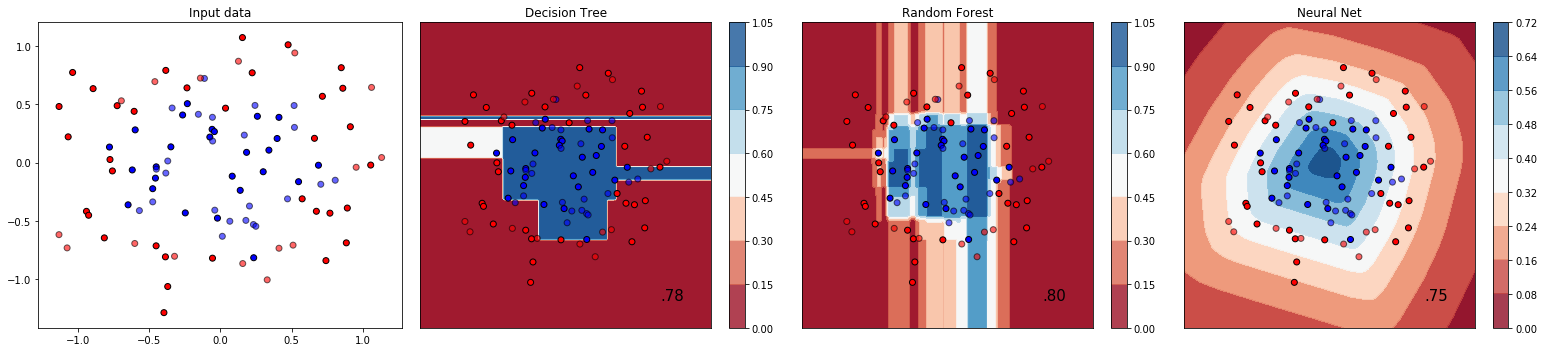
\includegraphics[width=1\linewidth]{image/C1.png}
\end{figure}
As we can observe, the classifiers have very high confidence in predictions  for input space at the corner even though no training data exists there. Therefore, our next plan is to design a method to identify the confident range of classifier based  on the principle that the models are only as good as the examples they have learned. As an toy example,  Figure~2 shows a contour plot after we classify the 2-d input space that has trained with the one that has not been trained. When the output is 0, it means the classifier has very low confidence.  In the next step, we plan derive an efficient solution to this problem  in high dimension space to help machine learning models avoid uncertain predictions that could result in hazard events.
\begin{figure}[h!]
  \label{fig:2}
  \caption{Classification with Unlearned Input Space}
  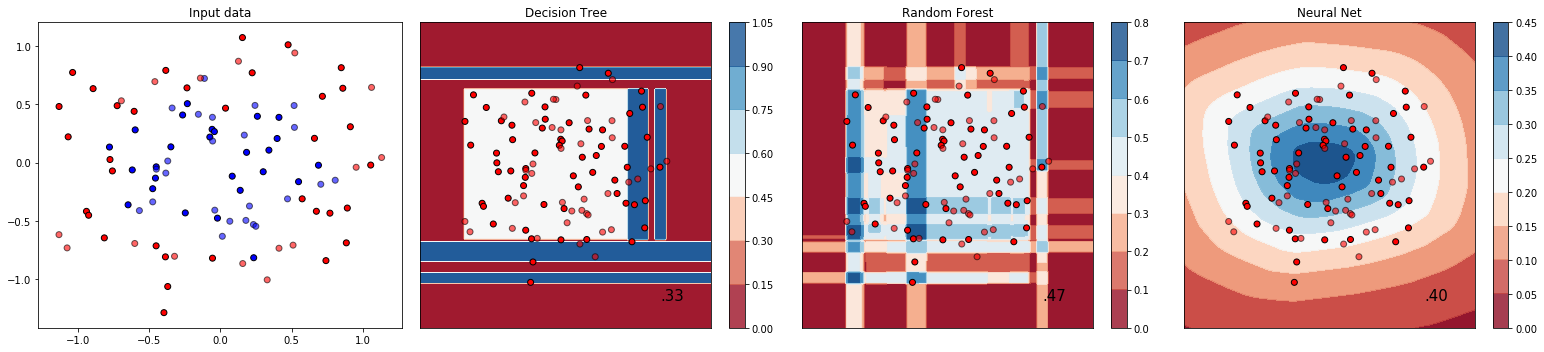
\includegraphics[width=1\linewidth]{image/C2.png}
\end{figure}



\renewcommand{\refname}{~}
\begin{thebibliography}{1}

\bibitem{safeml} Varshney KR, Alemzadeh H. On the safety of machine learning: Cyber-physical systems, decision sciences, and data products. Big data. 2017 Sep 1.



\bibitem{lime} Ribeiro, Marco Tulio, Sameer Singh, and Carlos Guestrin. Why should i trust you?: Explaining the predictions of any classifier. Proceedings of the 22nd ACM SIGKDD International Conference on Knowledge Discovery and Data Mining. ACM, 2016.


\bibitem{reject} Bartlett P L, Wegkamp M H. Classification with a reject option using a hinge loss[J]. Journal of Machine Learning Research, 2008, 9(Aug): 1823-1840.

\bibitem{errorbound} K. R. Varshney, R. J. Prenger, T. L. Marlatt, B. Y. Chen, and W. G. Hanley, Practical ensemble classification error bounds for different operating points, IEEE Transactions on Knowledge and Data Engineering, vol. 25, no. 11, pp. 2590-2601, Nov. 2013.
\bibitem{nntogp} Gal Y, Ghahramani Z. Dropout as a Bayesian approximation: Representing model uncertainty in deep learning[C]//international conference on machine learning. 2016: 1050-1059.

\bibitem{abstract} Tommaso Dreossi, Alexandre Donze,  Sanjit A. Seshia, Compositional Falsification of Cyber-Physical Systems with Machine Learning Components, Preprint

\bibitem{bnn12} Neal, R. M. (2012). Bayesian learning for neural networks (Vol. 118). Springer Science \& Business Media.
%

% \bibitem{Amodei} Amodei, Dario, Chris Olah, Jacob Steinhardt, Paul Christiano, John Schulman, and Dan Mane. 2016. Concrete Problems in AI Safety.

% \bibitem{Bostrom} Bostrom, N., Dafoe, A., and Flynn, C. 2016. Policy Desiderata in the Development of Machine Superintelligence


% \bibitem{conform} Vovk V, Gammerman A, Shafer G. Conformal prediction[M]. Springer US, 2005

% \bibitem{towardverify}  S. A. Seshia, D. Sadigh, and S. S. Sastry. Towards verified artificial intelligence. CoRR, abs/1606.08514, 2016.
 


% \bibitem{reduce} Weiming Xiang and Taylor T. Johnson, Reachability Analysis and Safety Verification for Neural  Network Control Systems,Preprint.


 



\end{thebibliography}


\end{document}
